%! TEX root = main.tex  % Specifies the main document file for multi-file projects

\chapter{Introduction to Computer Music Systems and Plugins}

\section{Learning Objectives}

This section covers fundamental concepts related to Computer Music Systems, including:

\begin{itemize}
    \item Understanding what a Computer Music Performance System (CMPS) is
    \item Learning the architecture of a CMPS
    \item Exploring the role of sequencers in the composition lifecycle
    \item Analyzing how signal processing systems operate within a sequencer
    \item Understanding how plugins function in a Digital Audio Workstation (DAW), including:
    \begin{itemize}
        \item GUI management
        \item Plugin API interaction
    \end{itemize}
\end{itemize}

\section{Applications of Computer Music Systems}

Computer music has evolved significantly due to progress in computer science and electronics. The main applications of computer music systems include:

\begin{itemize}
    \item Sound generation
    \item Automatic music composition
    \item Audio editing
    \item MIDI transmission, recording, and playback
    \item Sound processing
    \item Live sound processing
\end{itemize}

\section{Computer Music Performance Systems}

\begin{figure}[!htb]
    \centering
    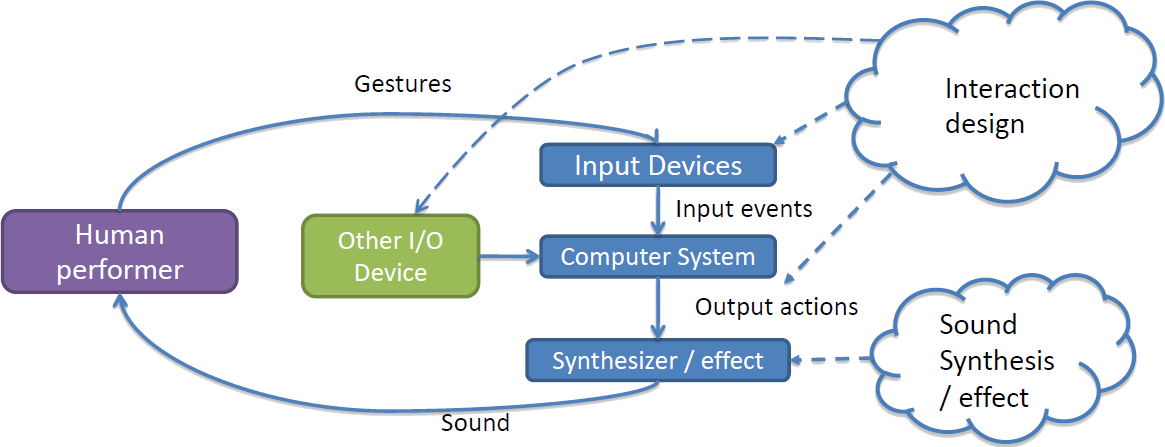
\includegraphics[width=0.8\linewidth]{00_Images/Res/05_chapter/01_cmps.png}
    \caption{Computer Music Performance System}
    \label{fig:computermusicperformancesystem}
\end{figure}

A Computer Music Performance System (CMPS) provides an interface between human performers and digitally controlled output devices. It consists of several key components:

\section{Components of a CMPS}

\begin{itemize}
    \item Human performer: Generates musical gestures while listening to the system’s output.
    \begin{itemize}
        \item Discrete gestures (e.g., pressing a key)
        \item Continuous gestures (e.g., varying pressure on a key)
    \end{itemize}
    \item Input device: Converts performance gestures into digital signals.
    \begin{itemize}
        \item Examples: computer keyboard, MIDI controller, motion sensors
    \end{itemize}
    \item Computer system: Processes input from devices and generates corresponding output actions.
    \begin{itemize}
        \item Can integrate additional input sources, such as external controllers
    \end{itemize}
    \item Synthesizer or effect processor: Receives commands from the computer system and generates or modifies audio waveforms.
\end{itemize}

\section{Applications of CMPS}

Computer Music Performance Systems enable various applications, including:

\begin{itemize}
    \item Virtual instruments
    \item Real-time composition
    \item Automated accompaniment
    \item Interactive performance environments
\end{itemize}

To support these applications, a CMPS must be programmable. The software environment of a CMPS typically includes:

\begin{itemize}
    \item One or more programming languages for defining musical interactions
    \item A real-time operating system that supports the semantic requirements of the language
\end{itemize}

\section{Real-Time Computer Music Systems}

A real-time system is one where system behavior depends on timing constraints. Real-time computer music systems must ensure low latency and precise timing for sound synthesis and interaction.

\section{Implementation of Computer Music Systems}

A computer music system consists of several interconnected components:

\paragraph{Hardware and Software Integration}

\begin{itemize}
    \item Personal Computer: The central processing unit for audio computation
    \item MIDI: Handles generation, recording, and playback of MIDI signals
    \item Audio: Manages sound synthesis, editing, recording, and playback
    \item Synthesizers: Can be implemented as:
    \begin{itemize}
        \item Software-based (internal)
        \item Hardware-based (external)
    \end{itemize}
\end{itemize}

\begin{figure}[!htb]
    \centering
    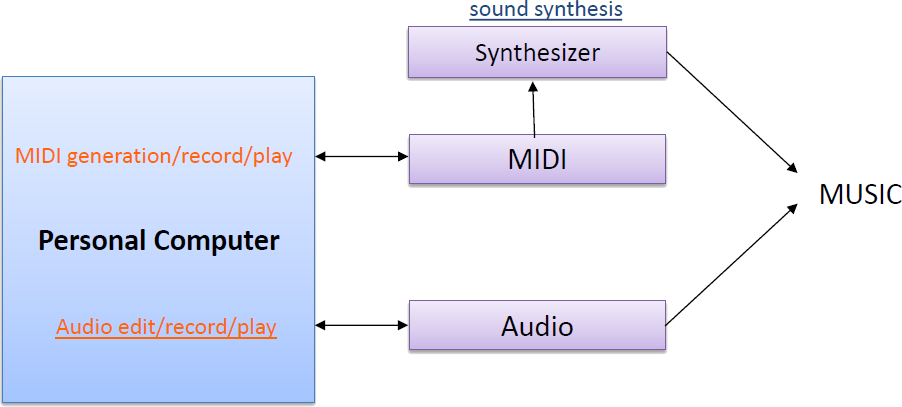
\includegraphics[width=0.8\linewidth]{00_Images/Res/05_chapter/02_cmsimplementation.png}
    \caption{Hardware and software integration}
    \label{fig:implementation01}
\end{figure}

\paragraph{System Architecture}

A computer music system includes multiple layers:

\begin{itemize}
    \item Software application: The user interface and main processing logic
    \item Kernel driver: Provides low-level access to audio hardware
    \item Sound card hardware: Processes and converts digital audio signals
    \item API and driver interaction: Manages communication between software and hardware
    \begin{itemize}
        \item Common APIs: PortAudio, PortMIDI, JACK, Core Audio
        \item Plugin standards: VST, Audio Unit
    \end{itemize}
\end{itemize}

\begin{figure}[!htb]
    \centering
    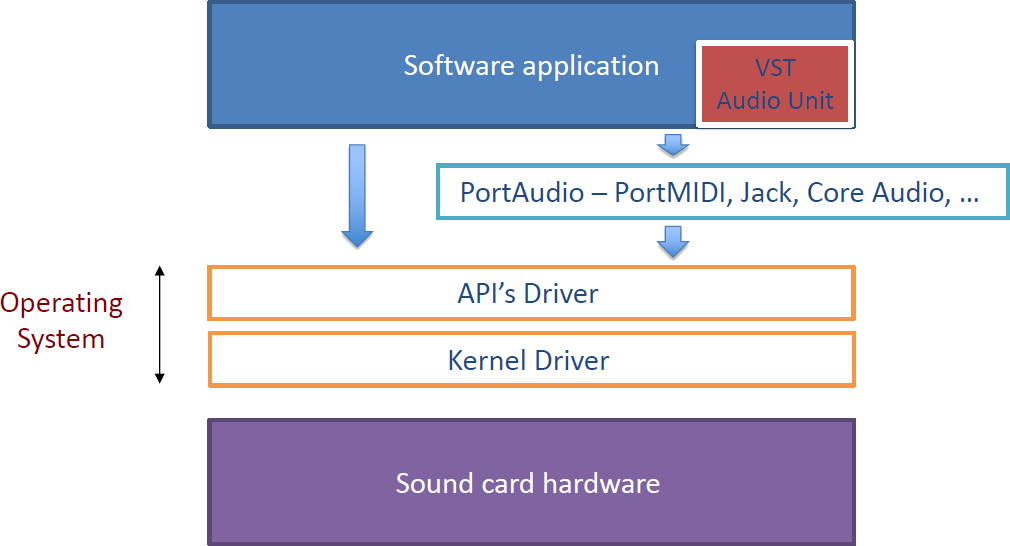
\includegraphics[width=0.8\linewidth]{00_Images/Res/05_chapter/03_cmsimplementation.png}
    \caption{System architecture}
    \label{fig:implementation02}
\end{figure}

\section{Sequencers and Their Role in Composition}

Sequencers play a fundamental role in the composition process by managing and organizing musical data. The composition process typically begins with MIDI (Musical Instrument Digital Interface) data, which consists of:

\begin{itemize}
    \item Notes
    \item Controller events
    \item Pitch bends
\end{itemize}

Modern sequencers allow for the recording of both MIDI data and digital audio from various sources, including:

\begin{itemize}
    \item MIDI devices (e.g., synthesizers, drum machines)
    \item Live instruments
    \item Vocal recordings
\end{itemize}

Once a musical project is stored as digital audio, it can be edited and processed with sound editing tools. Effects can be applied in real-time or offline to enhance the final output.

\subsection{Life-Cycle of a Composition in a Sequencer}

The composition process follows a structured flow:

\begin{enumerate}
    \item Musical data acquisition: Capturing notes, controller events, and pitch bends.
    \item Audio recording: Converting MIDI performances and live recordings into digital audio.
    \item Editing and processing: Modifying, arranging, and refining recorded material.
    \item Mixing and effects: Applying digital effects and balancing audio levels.
    \item Final rendering: Exporting the completed composition as a high-quality audio file.
\end{enumerate}

\begin{figure}[!htb]
    \centering
    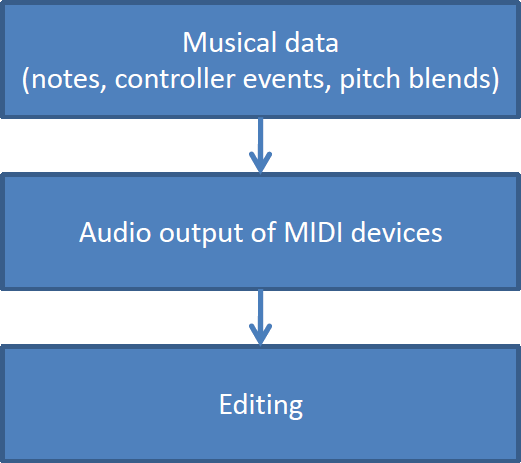
\includegraphics[width=0.7\linewidth]{00_Images/Res/05_chapter/04_sequencers.png}
    \caption{Life-cycle of a composition}
    \label{fig:life-cyclecomposition}
\end{figure}

\section{Signal Processing in Computer Music Systems}

Computer Music Performance Systems require efficient audio processing capabilities. Signal processing tasks can be divided into two categories:

\begin{itemize}
    \item Effect processing: Requires both input and output to modify an existing signal.
    \item Sound synthesis: Requires only an output to generate new sounds.
\end{itemize}

Signal processing systems integrate data acquisition hardware with microprocessors to execute algorithms on audio data. 

\begin{figure}[!htb]
    \centering
    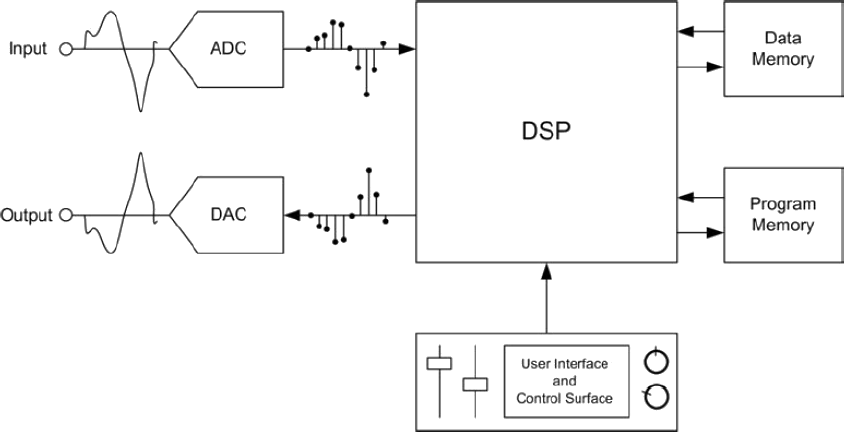
\includegraphics[width=0.8\linewidth]{00_Images/Res/05_chapter/05_signalprocessingsystem.png}
    \caption{Signal processing systems}
    \label{fig:signalprocessingsystems}
\end{figure}

\subsection{Effect Processor Architecture}

An effect processor typically consists of:

\begin{itemize}
    \item Digital Signal Processor (DSP): Specialized hardware optimized for real-time audio processing.
    \item User Interface (UI): Controls for modifying processing parameters, such as knobs and buttons.
    \item Program Memory: Stores the DSP program code.
    \item Data Memory: Stores input and processed audio data.
\end{itemize}

\subsection{DSP Execution Process}

DSPs operate efficiently by employing:

\begin{itemize}
    \item Multiply-and-accumulate operations as the core computational unit.
    \item Pipelining techniques to fetch new data while processing existing data.
\end{itemize}

\subsection{Music Synthesis Devices}

A music synthesis device is an embedded system that integrates a CPU and a DSP:

\begin{itemize}
    \item The microcontroller handles user input and controls.
    \item The DSP executes synthesis and effects algorithms.
\end{itemize}

\begin{figure}
    \centering
    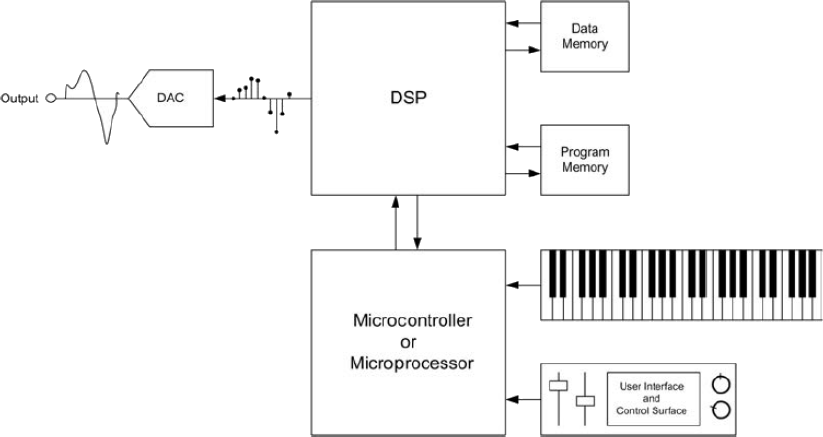
\includegraphics[width=0.8\linewidth]{00_Images/Res/05_chapter/06_signalprocessingsystem.png}
    \caption{Music synthesis system}
    \label{fig:musicsynthesissystem}
\end{figure}

\subsection{Signal Processing Flow}

The typical signal processing flow follows these steps:

\begin{enumerate}
    \item Initialization: Sets up the system and prepares for incoming data.
    \item Idle loop: Waits for an interrupt signal to process new data.
    \item Interrupt handling: Detects and decodes data interrupts.
    \item Data acquisition: Reads control and audio input data.
    \item Processing: Applies effects or synthesis algorithms to the audio signal.
    \item Output update: Adjusts parameters for the next processing cycle based on user input.
\end{enumerate}

Although traditionally performed on dedicated DSP hardware, this processing flow also applies to software-based implementations running on general-purpose computers.

\begin{figure}[!htb]
    \centering
    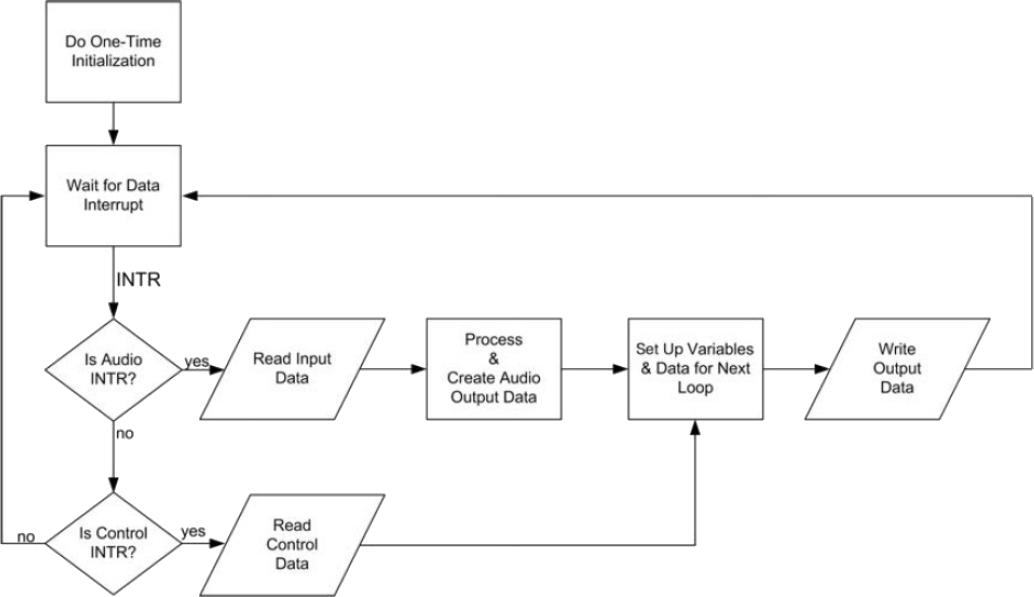
\includegraphics[width=0.8\linewidth]{00_Images/Res/05_chapter/07_signalprocessingflow.png}
    \caption{Signal processing flow}
    \label{fig:signalprocessingflow}
\end{figure}

\section{Plugins in Computer Music Systems}

A plugin is a software component that extends the functionality of another software application, referred to as the client. In computer audio systems, plugins serve various purposes, including:

\begin{itemize}
    \item Audio effects such as reverb, equalization, and distortion
    \item Signal analysis tools like oscilloscopes and spectrum analyzers
    \item Virtual instruments that function as synthesizers
\end{itemize}

\subsection{Interaction Between Plugins and the Client}

The communication method between a plugin and its client varies depending on the operating system:

\begin{itemize}
    \item Windows plugins are typically distributed as Dynamic Link Library (DLL) files.
    \item macOS plugins are packaged as bundles configured as components.
\end{itemize}

For simplicity, we refer to all dynamically linked plugins as DLLs.

\subsection{Static vs. Dynamic Linking}

\begin{itemize}
    \item Static linking: The plugin’s functions are compiled directly into the client application.
    \item Dynamic linking: The plugin exists as a separate file, and a communication mechanism is required to interact with the client.
\end{itemize}

Dynamic linking allows new functionalities to be added to a Digital Audio Workstation (DAW) without requiring recompilation.

\begin{figure}[!htb]
    \centering
    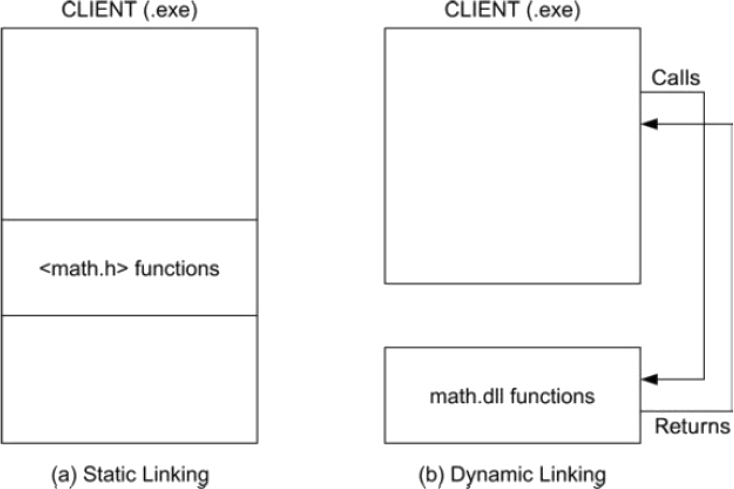
\includegraphics[width=0.6\linewidth]{00_Images/Res/05_chapter/08_plugins.png}
    \caption{Static vs. dynamic linking}
    \label{fig:staticdynamic}
\end{figure}

\subsection{Dynamic Link Library (DLL) Mechanism}

A DLL that shares the same process memory as the client requires the following steps to function:

\begin{enumerate}
    \item The client loads the DLL into its process address space.
    \item A communication mechanism is established between the client and the DLL functions.
    \item The client calls functions in the DLL as needed.
\end{enumerate}

In Windows, the following functions are used:

\begin{itemize}
    \item \texttt{LoadLibrary()}: Loads the DLL into memory.
    \item \texttt{GetProcAddress()}: Retrieves pointers to specific functions in the DLL.
    \item \texttt{FreeLibrary()}: Unloads the DLL when it is no longer needed.
\end{itemize}

\subsection{Implementation in C and C++}

\paragraph{C-style DLLs} In C, DLLs are implemented as collections of stand-alone functions without a \texttt{main()} function. To store persistent data:

\begin{itemize}
    \item A data structure is allocated using \texttt{malloc()} during initialization.
    \item A pointer to this structure is passed to the client for subsequent calls.
\end{itemize}

\begin{figure}[!htb]
    \centering
    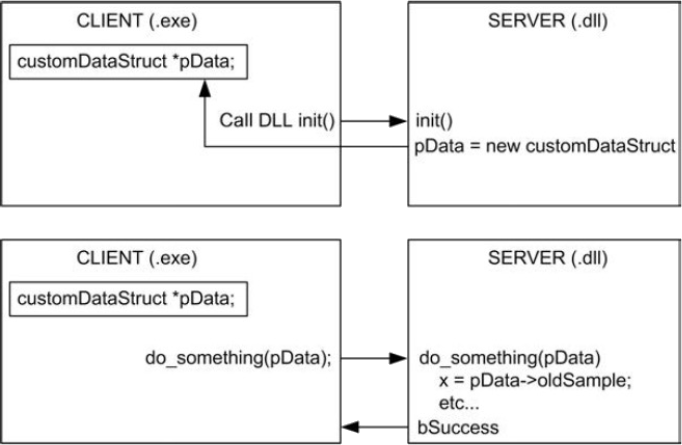
\includegraphics[width=0.6\linewidth]{00_Images/Res/05_chapter/09_plugins.png}
    \caption{C style DLL}
    \label{fig:cstyle}
\end{figure}

\paragraph{C++ style DLLs} In C++, DLLs take advantage of object-oriented programming:

\begin{itemize}
    \item Instead of allocating a data structure manually, the DLL creates an instance of a plugin object.
    \item The client interacts with the plugin by calling methods on this object.
    \item Multiple instances of the same plugin can be created and managed efficiently.
\end{itemize}

\begin{figure}[!htb]
    \centering
    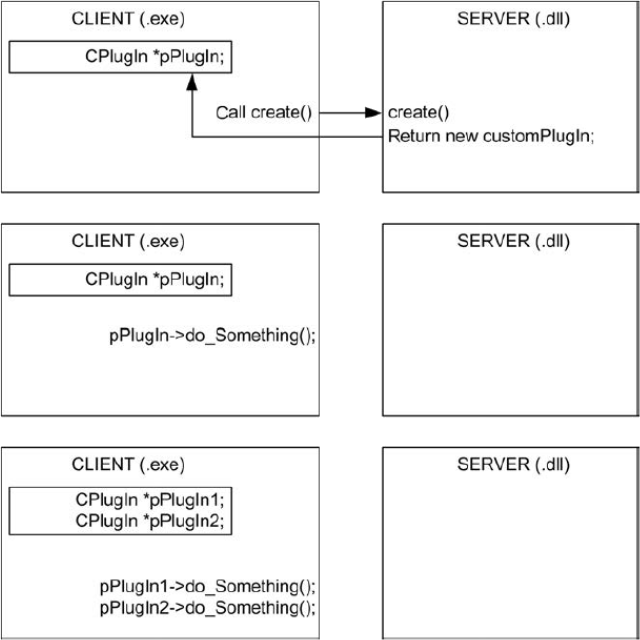
\includegraphics[width=0.6\linewidth]{00_Images/Res/05_chapter/10_plugins.png}
    \caption{C++ style DLL}
    \label{fig:c++style}
\end{figure}

\section{Graphical User Interface (GUI) for Plugins}

Most plugins include a GUI to control parameters. The GUI can be managed in three different ways:

\begin{enumerate}
    \item The client creates, maintains, and destroys the GUI, forwarding parameter changes to the plugin.
    \item The client creates and maintains the GUI, but the GUI directly communicates parameter changes to the plugin.
    \item The plugin itself handles the GUI and parameter communication.
\end{enumerate}

\subsection{GUI Management Strategies}

\paragraph{Client-Controlled GUI}

\begin{itemize}
    \item The client application is responsible for creating and managing the GUI.
    \item Control changes are forwarded to the plugin.
    \item This approach allows the client to have full control over GUI consistency.
\end{itemize}

\begin{figure}[!htb]
    \centering
    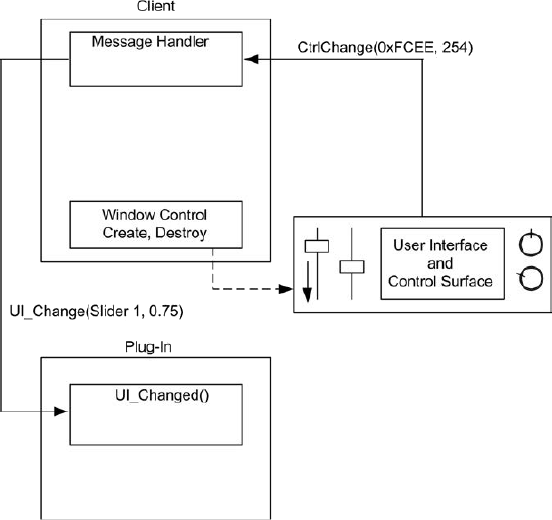
\includegraphics[width=0.6\linewidth]{00_Images/Res/05_chapter/11_userinterface.png}
    \caption{Client-controlled GUI}
    \label{fig:clientcontrolledgui}
\end{figure}

\paragraph{Client-Controlled GUI with Direct Plugin Communication}

\begin{itemize}
    \item The client creates the GUI but allows it to communicate directly with the plugin.
    \item This approach reduces the number of forwarded messages, improving efficiency.
\end{itemize}

\begin{figure}[!htb]
    \centering
    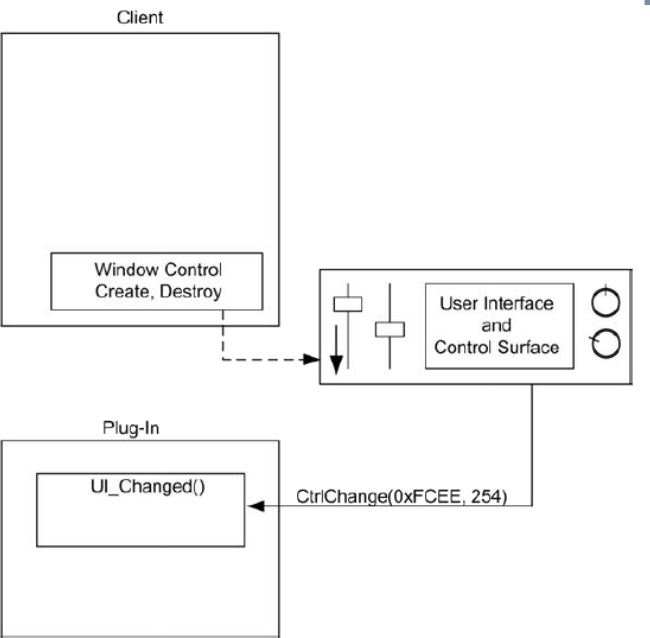
\includegraphics[width=0.6\linewidth]{00_Images/Res/05_chapter/12_userinterface.png}
    \caption{Client-controlled GUI with Direct Plugin Communication}
    \label{fig:clientcontrolledguiwithdirectplugincomm}
\end{figure}

\paragraph{Plugin-Controlled GUI}

\begin{itemize}
    \item The plugin creates and manages its own GUI.
    \item This provides more flexibility but requires the plugin to handle GUI updates and interactions.
\end{itemize}

\begin{figure}[!htb]
    \centering
    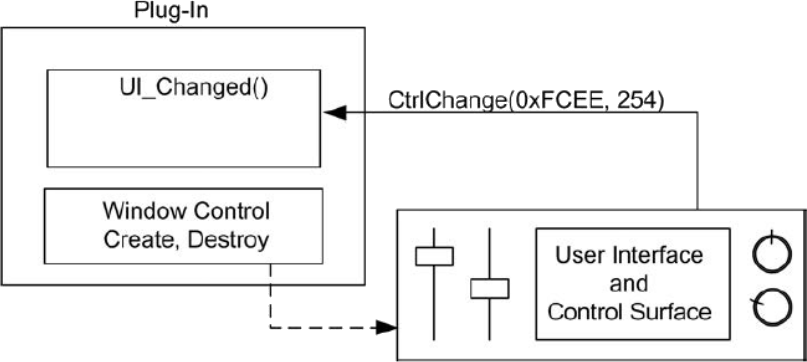
\includegraphics[width=0.6\linewidth]{00_Images/Res/05_chapter/13_userinterface.png}
    \caption{Plugin-controlled GUI}
    \label{fig:plugincontrolledgui}
\end{figure}

\section{Plugin Structure and API}

A plugin must implement a minimal set of functions defined by the Application Programming Interface (API) to interact with the client. The API ensures:

\begin{itemize}
    \item Compatibility across different versions of the client software.
    \item A standardized set of functions that all plugins must implement.
\end{itemize}

Object-oriented programming simplifies API integration:

\begin{itemize}
    \item If the plugin is an instance of an abstract base class defined by the client manufacturer, the API functions are guaranteed to be implemented.
\end{itemize}

\subsection{Core Plugin Operations}

Common functions shared across plugin APIs include:

\begin{itemize}
    \item Initialization and shutdown
    \item Audio processing
    \item Parameter management
    \item GUI handling
\end{itemize}